%% ut-thesis.tex -- document template for graduate theses at UofT
%%
%% Copyright (c) 1998-2013 Francois Pitt <fpitt@cs.utoronto.ca>
%% last updated at 16:20 (EDT) on Wed 25 Sep 2013
%%
%% This work may be distributed and/or modified under the conditions of
%% the LaTeX Project Public License, either version 1.3c of this license
%% or (at your option) any later version.
%% The latest version of this license is in
%%     http://www.latex-project.org/lppl.txt
%% and version 1.3c or later is part of all distributions of LaTeX
%% version 2005/12/01 or later.
%%
%% This work has the LPPL maintenance status "maintained".
%%
%% The Current Maintainer of this work is
%% Francois Pitt <fpitt@cs.utoronto.ca>.
%%
%% This work consists of the files listed in the accompanying README.

%% SUMMARY OF FEATURES:
%%
%% All environments, commands, and options provided by the `ut-thesis'
%% class will be described below, at the point where they should appear
%% in the document.  See the file `ut-thesis.cls' for more details.
%%
%% To explicitly set the pagestyle of any blank page inserted with
%% \cleardoublepage, use one of \clearemptydoublepage,
%% \clearplaindoublepage, \clearthesisdoublepage, or
%% \clearstandarddoublepage (to use the style currently in effect).
%%
%% For single-spaced quotes or quotations, use the `longquote' and
%% `longquotation' environments.


%%%%%%%%%%%%         PREAMBLE         %%%%%%%%%%%%

%%  - Default settings format a final copy (single-sided, normal
%%    margins, one-and-a-half-spaced with single-spaced notes).
%%  - For a rough copy (double-sided, normal margins, double-spaced,
%%    with the word "DRAFT" printed at each corner of every page), use
%%    the `draft' option.
%%  - The default global line spacing can be changed with one of the
%%    options `singlespaced', `onehalfspaced', or `doublespaced'.
%%  - Footnotes and marginal notes are all single-spaced by default, but
%%    can be made to have the same spacing as the rest of the document
%%    by using the option `standardspacednotes'.
%%  - The size of the margins can be changed with one of the options:
%%     . `narrowmargins' (1 1/4" left, 3/4" others),
%%     . `normalmargins' (1 1/4" left, 1" others),
%%     . `widemargins' (1 1/4" all),
%%     . `extrawidemargins' (1 1/2" all).
%%  - The pagestyle of "cleared" pages (empty pages inserted in
%%    two-sided documents to put the next page on the right-hand side)
%%    can be set with one of the options `cleardoublepagestyleempty',
%%    `cleardoublepagestyleplain', or `cleardoublepagestylestandard'.
%%  - Any other standard option for the `report' document class can be
%%    used to override the default or draft settings (such as `10pt',
%%    `11pt', `12pt'), and standard LaTeX packages can be used to
%%    further customize the layout and/or formatting of the document.

%% *** Add any desired options. ***
\documentclass{ut-thesis}

%% *** Add \usepackage declarations here. ***
%% The standard packages `geometry' and `setspace' are already loaded by
%% `ut-thesis' -- see their documentation for details of the features
%% they provide.  In particular, you may use the \geometry command here
%% to adjust the margins if none of the ut-thesis options are suitable
%% (see the `geometry' package for details).  You may also use the
%% \setstretch command to set the line spacing to a value other than
%% single, one-and-a-half, or double spaced (see the `setspace' package
%% for details).

%%%%%%%%%%%%%%%%%%%%%%%%%%%%%%%%%%%%%%%%%%%%%%%%%%%%%%%%%%%%%%%%%%%%%%%%
%%                                                                    %%
%%                   ***   I M P O R T A N T   ***                    %%
%%                                                                    %%
%%  Fill in the following fields with the required information:       %%
%%   - \degree{...}       name of the degree obtained                 %%
%%   - \department{...}   name of the graduate department             %%
%%   - \gradyear{...}     year of graduation                          %%
%%   - \author{...}       name of the author                          %%
%%   - \title{...}        title of the thesis                         %%
%%%%%%%%%%%%%%%%%%%%%%%%%%%%%%%%%%%%%%%%%%%%%%%%%%%%%%%%%%%%%%%%%%%%%%%%

%% *** Change this example to appropriate values. ***
\degree{Master of Applied Science}
\department{Civil Engineering}
\gradyear{2019}
\author{Stepan Oskin}
\title{Design and implementation of a housing market database for Greater Toronto and Hamilton area.
Part of a Longitudinal Analysis of housing sales in the Greater Toronto-Hamilton Area.}


%% *** NOTE ***
%% Put here all other formatting commands that belong in the preamble.
%% In particular, you should put all of your \newcommand's,
%% \newenvironment's, \newtheorem's, etc. (in other words, all the
%% global definitions that you will need throughout your thesis) in a
%% separate file and use "\input{filename}" to input it here.


%% *** Adjust the following settings as desired. ***

%% List only down to subsections in the table of contents;
%% 0=chapter, 1=section, 2=subsection, 3=subsubsection, etc.
\setcounter{tocdepth}{2}

%% Make each page fill up the entire page.
\flushbottom


%%%%%%%%%%%%      MAIN  DOCUMENT      %%%%%%%%%%%%

\begin{document}

%% This sets the page style and numbering for preliminary sections.
\begin{preliminary}

%% This generates the title page from the information given above.
\maketitle

%% There should be NOTHING between the title page and abstract.
%% However, if your document is two-sided and you want the abstract
%% _not_ to appear on the back of the title page, then uncomment the
%% following line.
%\cleardoublepage

%% This generates the abstract page, with the line spacing adjusted
%% according to SGS guidelines.
\begin{abstract}
%% *** Put your Abstract here. ***
%% (At most 150 words for M.Sc. or 350 words for Ph.D.)
    Teranet dataset of real estate transactions recorded in the Province of Ontario holds a wealth of information on the housing market of Ontario, but is very limited in the number of available attributes.
    The dataset can be augmented by joining additional attributes from various data sources, such as Census or TTS survey, based on spatial and/or temporal relationships.
    These relationships are best organized in the form of a relational database based on a database management system, such as PostgreSQL .
    Primary focus of this master's thesis is design and implementation of the proposed GTHA housing market database.
\end{abstract}

%% Anything placed between the abstract and table of contents will
%% appear on a separate page since the abstract ends with \newpage and
%% the table of contents starts with \clearpage.  Use \cleardoublepage
%% for anything that you want to appear on a right-hand page.

%% This generates a "dedication" section, if needed -- just a paragraph
%% formatted flush right (uncomment to have it appear in the document).
%\begin{dedication}
%% *** Put your Dedication here. ***
%\end{dedication}

%% The `dedication' and `acknowledgements' sections do not create new
%% pages so if you want the two sections to appear on separate pages,
%% uncomment the following line.
%\newpage  % separate pages for dedication and acknowledgements

%% Alternatively, if you leave both on the same page, it is probably a
%% good idea to add a bit of extra vertical space in between the two --
%% for example, as follows (adjust as desired).
%\vspace{.5in}  % vertical space between dedication and acknowledgements

%% This generates an "acknowledgements" section, if needed
%% (uncomment to have it appear in the document).
%\begin{acknowledgements}
%% *** Put your Acknowledgements here. ***
%\end{acknowledgements}

%% This generates the Table of Contents (on a separate page).
\tableofcontents

%% This generates the List of Tables (on a separate page), if needed
%% (uncomment to have it appear in the document).
%\listoftables

%% This generates the List of Figures (on a separate page), if needed
%% (uncomment to have it appear in the document).
%\listoffigures

%% You can add commands here to generate any other material that belongs
%% in the head matter (for example, List of Plates, Index of Symbols, or
%% List of Appendices).

%% End of the preliminary sections: reset page style and numbering.
\end{preliminary}


%%%%%%%%%%%%%%%%%%%%%%%%%%%%%%%%%%%%%%%%%%%%%%%%%%%%%%%%%%%%%%%%%%%%%%%%
%%  Put your Chapters here; the easiest way to do this is to keep     %%
%%  each chapter in a separate file and `\include' all the files.     %%
%%  Each chapter file should start with "\chapter{ChapterName}".      %%
%%  Note that using `\include' instead of `\input' will make each     %%
%%  chapter start on a new page, and allow you to format only parts   %%
%%  of your thesis at a time by using `\includeonly'.                 %%
%%%%%%%%%%%%%%%%%%%%%%%%%%%%%%%%%%%%%%%%%%%%%%%%%%%%%%%%%%%%%%%%%%%%%%%%

%% *** Include chapter files here. ***
\chapter[Introduction]{Introduction} \label{ch:introduction}

\section{Introduction} \label{sec:intro}
\chapter[Background information]{Background information} \label{ch:background}

\section{Chapter 2: transportation and land use, land registration in Canada and Teranet} \label{sec:chapter_2_intro}

This chapter discusses the complex interaction of land use and transportation, provides a brief overview of the history of development of land use-transportation (LUT) models, presents some legal and historical background for Teranet's dataset of real estate transactions and finishes with discussing challenges of working with Teranet's data and the proposed solution.

\section{Land Use and Transport (LUT) models} \label{sec:evolution_of_models_of_urban_systems}

\subsection{Complexity of urban systems and "wicked" problems} \label{subsec:complexity_and_wicked_problems}

In her famous 1961 book, Jane Jacobs\cite{Jacobs1961} described a city as "a problem in organized complexity";
since then, many other researchers have remarked that urban systems exhibit complex behaviour\cite{Batty2008, Bettencourt2013}.
Complexity of a system can be defined as a state or quality of being intricate or complicated.
For a system to be complex is not necessarily the same as to be complicated;
complex systems can be simple, i.e.\ governed by a single equation.
Complexity of a system has to do with the intrinsic ability of a system to surprise us with its behaviour;
that the system is hard to understand, despite the mechanics of it being relatively simple.

In 1973, a little over a decade after Jacobs, Rittel and Webber\cite{Rittel1973} presented a path-breaking conceptualization;
this conceptualization characterized urban planning problems as "wicked" problems: problems which cannot be definitively described and for which it makes no sense to talk of "optimal solutions".
In their paper, Rittel and Webber stated that such "wicked" problems are never "solved", and that the focus instead becomes on iteratively "re-solving" the problems over and over.
More than 40 years after their original publication, Rittel and Webber's ideas remain relevant to the policy sciences today: there is an intense interest in the nature of "wicked" problems and the complex tasks of identifying their scope, viable responses, and appropriate mechanisms and pathways to improvement\cite{Crowley2017}.
Interaction between land use and transportation, which is discussed in the following section, presents a prime example of urban complexities and "wicked" problems.

\subsection{Transportation-land use cycle} \label{subsec:transportation_land_use_cycle}

Among the reasons why transportation and land use interaction is "wicked" are such aspects as pluralism of expectations among stakeholders, institutional complexity in policy making, and scientific uncertainty\cite{Noto2015}.
More importantly, there is a fundamental link between transportation and urban form: urban form has an enormous impact on the type and cost of transportation systems needed to serve residents of a metropolitan area\cite{Kelly1994}.
Transportation, in turn, influences land development and location choices of people and firms, and thus completes the formation of a feedback relationship that Stover and Koepke\cite{Stover1988} referred to as a cycle.
Interconnections between points (activities) in space can be perceived through the medium of the transportation system\cite{Miller1998}

Figure~\ref{fig:idealized_integrated_urban_model} illustrates the complex interactions between land use and transportation system as summarized by Miller, Kriger and Hunt\cite{Miller1998}.

\begin{figure}[hbt!]
    \centering
    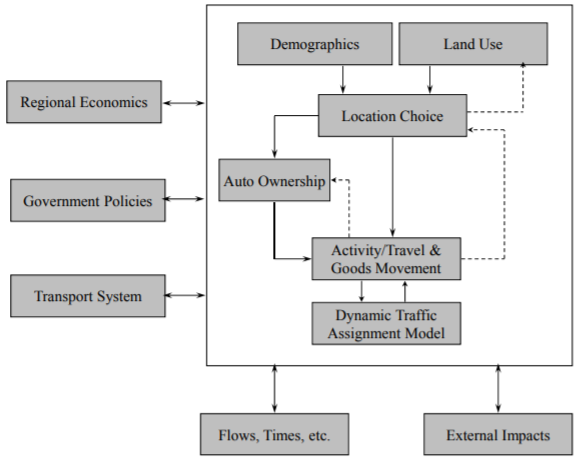
\includegraphics[width=0.7\linewidth,trim=0 0 0 0,clip]{miller_idealized_urban_model.png}
    \caption{An Idealized Integrated Urban Model System, adapted from Miller, Kriger and Hunt\cite{Miller1998}.}
    \label{fig:idealized_integrated_urban_model}
\end{figure}

Many different types of models are used in planning, such as demand forecasting models projecting traffic or ridership, or land use models projecting and distributing population and jobs within an area.
At an earlier stage of model development, some analysts argued that there is no significant link between transportation and land use, given the near-ubiquity of the transportation (road) network\cite{Miller1998}.
However, the unprecedented urban growth of the 21st century introduced new challenges for urban systems such as extreme road congestion, equity of access to jobs and services among low-income households, energy scarcity, environmental and GHG impacts from transportation systems and public health impacts of land use patterns\cite{Miller2018b,Moeckel2017}.

It became apparent that these "transport problems" cannot be solved through transportation policies and investment alone, that the physical design of the city at the "macro" and "micro" scale critically interfaces with the demand for and performance of the transportation system.
In addition, to accurately assess the costs and benefits of an expensive long-term transportation infrastructure investment, "feedback" effects of these investments on urban form, land values, property taxes, quality of life, etc.
need to be quantified and included in evaluation and decision making.
Thus, today there is a steadily growing recognition within the urban policy field that the interaction between transportation and land use does exist and does matter\cite{Miller2018b}.

%TODO change the end of 1st sentence
In the context of models, integrated urban models (IUMs) aim to capture the complex relationship between urban systems such as transportation and land use more accurately.
Integrated land use-transportation models combine travel demand forecasting and land use forecasting functions and recognize that the distribution of population and jobs depends, in part, on transportation accessibility.
The reverse is also true, and thus integrated models incorporate feedback relationship between transportation and land use, with economic decisions by households and firms acting as one of the links between the two systems\cite{Miller1998}.

\subsection{Evolution of LUT models} \label{subsec:evolution_of_lut_models}

The history of treating cities as systems via simulation models of transportation and land use dates back to 1950s when General System Theory and Cybernetics came to be applied in the softer social sciences\cite{Batty2008}.
The first operational simulation model that truly integrated land use and transportation is considered to be A Model of Metropolis built in 1964 by Ira S. Lowry for the Pittsburgh region based on economic base theory\cite{Lowry1964}.
It was a highly aggregate model based on theories of spatial interaction, such as the gravity model that was popular in quantitative geography and transportation planning at the time\cite{Bouchard1965}.
Models based on spatial interaction framework continued to be developed through mid-1980s, until developments in random utility theory allowed researchers to describe choices among discrete alternatives, such as the choice of travel mode, and generate models based on the study of disaggregate behaviour\cite{Iacono2008}.

Figure~\ref{fig:lut_model_evolution} provides the general overview of chronological development of LUT models summarized by Iacono\cite{Iacono2008}.

\begin{figure}[hbt!]
    \centering
    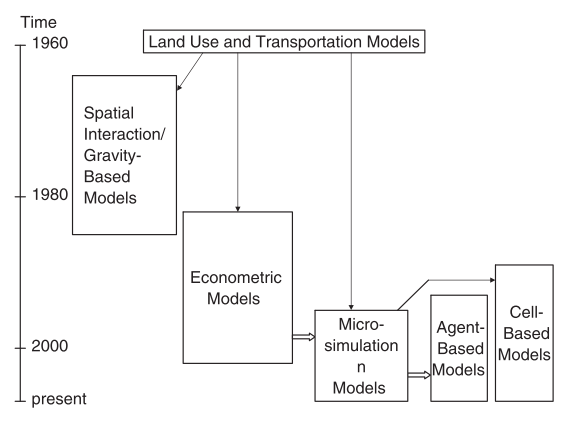
\includegraphics[width=0.7\linewidth,trim=0 0 0 0,clip]{lut_models_evolution.png}
    \caption{Chronological development of LUT models summarized by Iacono\cite{Iacono2008}.}
    \label{fig:lut_model_evolution}
\end{figure}

The modeling paradigm has changed fundamentally in the early 1990s along with the advances in computing power and efficiency of data storage.
Urban systems used to be viewed as hierarchical and centrally organized equilibrium structures, or "top-down".
Instead, now they were considered to be structured from the "bottom-up", dynamically retaining their integrity through interactions of numerous microelements\cite{Batty2008}.
A new broad class of LUT models that could fall under the title of "microsimulation" began to be developed.
It included such classes of models as activity-based travel, cell-based models, and multi-agent models, and more recently comprehensive urban microsimulation models that fully reflect the dynamics of changes in the population and the urban environment\cite{Iacono2008}.
%TODO check last sentence

"Micro" in the microsimulation implies that the model must be highly disaggregated spatially, socio-economically and in its representation of processes.
"Simulation" implies that the model must be numerical, stochastic, have an explicit time dimension, and "evolve" into the end state rather than "solve for it"\cite{Miller2018c}.
An example of such model has been developed by the University of Toronto ILUTE team;
their product is an integrated urban model capable of microsimulating urban demographic evolution, housing markets and travel behaviour over extended periods of time\cite{Miller2018a}.
The ILUTE system and some of the ways for its future improvement are discussed in the following section.

\subsection{ILUTE and HoMES model systems} \label{subsec:ilute}

The Integrated Land Use, Transportation, Environment (ILUTE) model system is an agent-based microsimulation model for greater Toronto-Hamilton area;
it includes such components as land use, activity/travel, urban economics, auto ownership, demographics and emissions/energy use.
It uses disaggregate models of spatial socioeconomic processes to evolve the state of the greater Toronto\textendash Hamilton area from a known base case to a predicted end state in 1-year time steps.
The system state is defined in terms of the individual persons, households, dwelling units, firms, etc.
that collectively define the urban region being modeled\cite{Miller2011}.

ILUTE model simulates the evolution of an urban region's spatial form, demographics, travel behavior and economic structure over time.
Many markets are of interest within ILUTE, such as housing, labour, commercial, real estate, etc.) and are modeled via microsimulation.
The model aims to capture the dynamics of these markets through disaggregated representations.
For example, in the housing market component of ILUTE, houses are auctioned off one dwelling at a time to interested bidders in a disaggregate implementation of Martinez' Bid Choice theory\cite{Martinez1992}.

The Housing Market Evolutionary System (HoMES) is the updated housing market module for the ILUTE model system.
HoMES is a disaggregate, agent-based microsimulation of the owner-occupied housing market that evolves the residential location of households over time and includes the endogenous supply of housing by type and location, as well as the endogenous determination of sales prices and rents.

An overview of the framework of housing market supply, demand and clearing mechanisms utilized in HoMES provided by Rosenfield et al.\cite{Rosenfield2013} is presented on figure~\ref{fig:homes_framework}

\begin{figure}[hbt!]
    \centering
    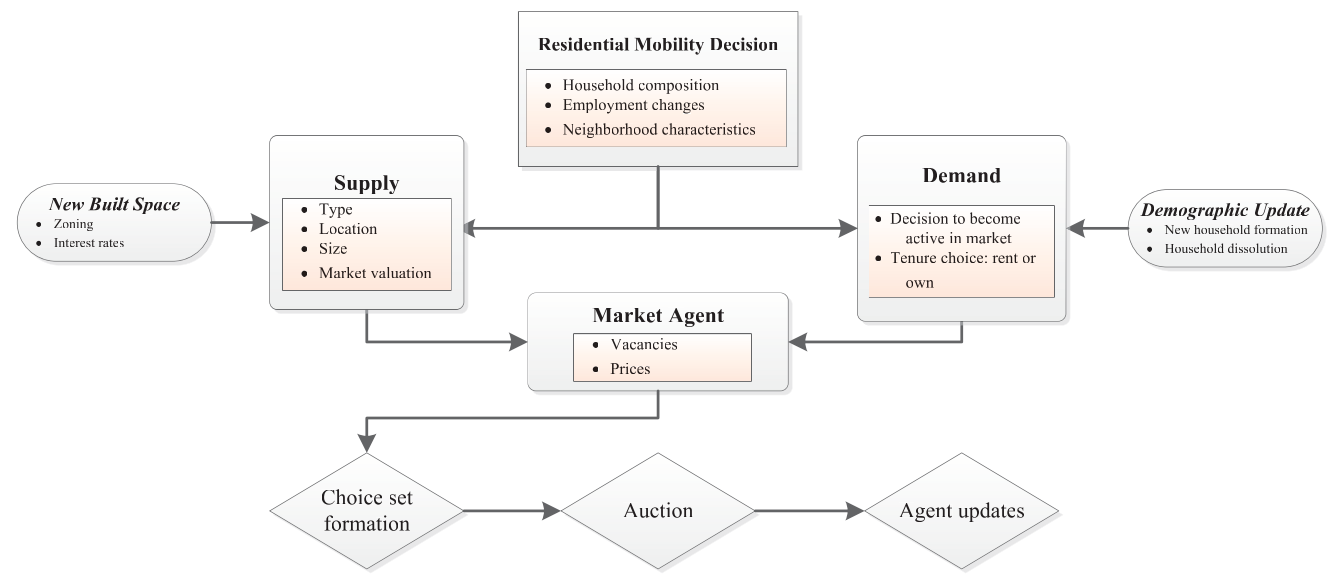
\includegraphics[width=0.99\linewidth,trim=0 0 0 0,clip]{homes_framework.png}
    \caption{Framework of housing market supply, demand and clearing mechanisms used in HoMES module of ILUTE, as summarized by Rosenfield et al.\cite{Rosenfield2013}.}
    \label{fig:homes_framework}
\end{figure}

Among the major barriers to implementation of integrated urban models since their introduction were such aspects as data hungriness and computational requirements\cite{Miller1998}.
However, continuing methodological advances, such as cost-effective High Performance Computing (HPC), detailed GIS-based datasets and machine learning methods, mean that former barriers now represent opportunities for model system development.
In the case of ILUTE and HoMES, one of the possibilities for further improvement is the use of new data sources to update the housing market model.
One of these new data sources, Teranet's dataset of land registry records, and main challenges of working with it are discussed in section~\ref{sec:new_data_sources_and_their_challgenges}.

\section{New data sources and their challenges} \label{sec:new_data_sources_and_their_challgenges}

\subsection{Further improvement of integrated urban models} \label{subsec:further_improvement_of_iums}


As an increasing amount of aspects of human life becomes digitalized, a wealth of new data is produced and can be used to model and analyze dynamics of urban systems\cite{Arribas-Bel2014, Chen2016}.
An example of such digitalization of human activity is the introduction of the Province of Ontario Land Registration Information System (POLARIS) in 1985 by the Government of Ontario\cite{TeranetEnterprisesInc.} that will be discussed in the following section.
Introduction of POLARIS lead to the creation of an extensive dataset of real estate transactions (land registration records) by the Teranet Enterprises Inc.
This dataset offers a very fine resolution of housing market dynamics across both time and space, which can be beneficial for updating and testing microsimulation models, but it also presents challenges to work with that will be discussed in section~\ref{subsec:teranet_ontario} of this chapter;
the chapter concludes with the proposed solution to address one of the main challenges of working with Teranet's data.

\subsection{POLARIS: electronic system of land registration in Ontario} \label{subsec:land_reg_system_canada}

All land owned in Canada is registered in a public land registry in the applicable province.
Each province and territory in Canada has its own land registry system, whether it is a land titles system, a registry system or a combination of both, with each system having its own rules.
The registry system is a public record of documents evidencing transactions affecting land.
In the land titles system, the applicable provincial government determines the quality of the title, and essentially guarantees (within certain statutory limits) the title to, and interests in, the property.
As of 2015, most common law provinces and territories in Canada were using the land titles system or were in the process of converting from a registry system to a land titles system\cite{McKean2015}.

As of 2015, the Province of Ontario has largely converted from registry systems to a land titles system.
In 1985, the Government of Ontario initiated the Province of Ontario Land Registration Information System (POLARIS) pilot project for the purposes of the conversion between systems and records automation.
The Land Registration Reform Act (Ontario)\cite{TheGovernmentofOntario1990} was introduced in 1990 to facilitate electronic search and registration of properties and the automation of paper-based records.
POLARIS was built by the Province to house and process electronic land records, which in turn lead to the creation of an extensive dataset of land registration records managed by Teranet Enterprises Inc.
Today, POLARIS is the search/registration and property maintenance system for all automated land records in Ontario.

\subsection{The Teranet-Ontario Partnership, Teranet's data and its challenges} \label{subsec:teranet_ontario}

In 1991, the Government of Ontario established a partnership with Teranet, a Toronto-based organization, founded the same year, which provides e-services to legal, real estate, government, financial, and healthcare markets.
The partnership was established to convert Ontario's land registration system to a more modernized electronic title system.
The project involved taking a 200-year-old paper-based system and creating a database with electronic records for more than five million parcels of land.
Teranet converted all qualified Registry properties in Ontario to the Land Titles system and automated existing paper Land Titles parcels.
As a result, 99.9\% of property in Ontario was parcelized and administered under the Land Titles system.
Teranet fully automated the conversion of millions of paper-based documents and records into the Ontario Electronic Land Registration System (ELRS)\cite{TeranetEnterprisesInc.2019}.


Teranet dataset presents an extensive historical record of real estate transactions recorded in the Province of Ontario since the beginning of XIX century.
However, when it comes to using new data sources in social studies, along with opportunities there are also challenges present.
For example, these data sources can have issues with the quality of the data, might require a specific set of skills to take advantage of these data sources, or might not be suitable for traditional methods meant for traditional data\cite{Arribas-Bel2014}, all of which are true in the case of Teranet's dataset.

One of the major attributes missing from the available version of Teranet's dataset is the information about the type of property being transacted, with records of various residential, commercial and industrial properties all being mixed together in the same dataset.
At the same time, Teranet records have timestamps (dates) and location information (x and y coordinates) and thus can be joined to variety of other urban data sources, such as Census demographics, Transportation Tomorrow Survey (TTS) and parcel-level land use information.
It is possible to derive this attribute from additional related sources of information, such as detailed land use or Census demographics.
However, joining these data sources together requires additional considerations, as they use different spatial units and are available at different temporal spans, as will be discussed in chapter~\ref{ch:spatial_and_temporal_relationships_between_urban_data}.


\section{Chapter summary} \label{sec:background_summary}

The fundamental link between transportation and urban form creates a feedback relationship between land development, travel needs, viability of alternative modes, accessibility, and other important characteristics of the urban transportation system.
Numerous "top-down" and "bottom-up" models have been designed to analyze and forecast the behaviour of urban regions and interaction of their transportation and land use systems.
Since urban systems are complex in nature and require "re-solving" over and over, data science process models present a good fit for this task with their iterative structure.

Increased digitization of human activity, such as introduction of POLARIS land registration system by the Government of Ontario in 1985, produce a wealth of new information that can be used to study interaction between land use and transportation at a fine spatial and temporal scale.
Teranet's dataset of real estate transactions presents a wealth of information on the housing market of Ontario and can be used for empirical studies of transportation-land use interaction.
However, along with the opportunities, the new data sources also present new challenges.
Teranet's dataset has some data quality issues that need to be addressed and might require special skills to work with due to its size.
But most importantly, it is very limited in the number of features available for each transaction.

One of the major attributes missing from the available version of Teranet's dataset is the information about the type of property being transacted, with records of various residential, commercial and industrial properties all being mixed together in the same dataset.
At the same time, Teranet records have timestamps (dates) and location information (x and y coordinates) and thus can be joined to variety of other urban data sources, such as Census demographics, Transportation Tomorrow Survey (TTS) and parcel-level land use information.
It is possible to derive this attribute from additional related sources of information, such as detailed land use or Census demographics.
However, joining these data sources together requires additional considerations, as they use different spatial units and are available at different temporal spans, as will be discussed in chapter~\ref{ch:spatial_and_temporal_relationships_between_urban_data}.

\chapter{Description of Teranet's dataset} \label{ch:teranet}

\section{Introduction: Teranet's dataset of land registration records} \label{sec:intro_teranet}

%TODO add chapter introduction

This section describes the systems of registration for land and real estate sales utilized in Canada and the Province of Ontario, brief history of their development, overview of their main features, and the role played by the Teranet Enterprises Inc.
in maintaining and providing access to land registry in Ontario.

\subsection{System of land registration in Canada} \label{subsec:land_reg_system_canada}

According to Chapter 6 of the International Comparative Legal Guide to Real Estate published by the Global Legal Group in 2015\cite{McKean2015}, all land owned in Canada is registered in a public land registry through either a registry system, a land titles system or a combination of both in the applicable province.
The registry system is a public record of documents evidencing transactions affecting land.
In the land titles system, the applicable provincial government determines the quality of the title, and essentially guarantees (within certain important statutory limits) the title to, and interests in, the property.
As of 2015, most common law provinces and territories were using the land titles system or were in the process of converting title from a registry system to a land titles system.

On the purchase and sale of real estate and land, ownership is generally transferred to the buyer when the deed or transfer is registered in the applicable land registry office.
An agreement of purchase and sale must be in writing to be enforceable.
A transfer of ownership is actualised by registering, either physically or electronically (depending on the applicable land registry system), a deed or transfer with the applicable land registry office or land registrar, copies of which can be obtained from the relevant registry office, often electronically.

Once registration is complete, a copy of the transfer (if in the land titles system) or deed (if in the registry system) or a copy of a certificate of title is issued to the owner to confirm the registration and status of title.

\subsection{POLARIS: Land registration system of Ontario} \label{subsec:lang_reg_operating_canada}

Each province and territory in Canada has its own land registry system, whether it is a land titles system, a registry system or a combination of both, with each system having its own rules.
As of 2015, the Province of Ontario has largely converted from registry systems to a land titles system.

In 1985, the Government of Ontario initiated the \textbf{Province of Ontario Land Registration Information System (POLARIS)} pilot project for the purposes of records automation and the conversion from the Registry System to the Land Titles System.
The \textit{Land Registration Reform Act (Ontario)}\cite{TheGovernmentofOntario1990} was introduced in 1990 to facilitate electronic search and registration of properties and the automation of paper-based records.
POLARIS was built by the Province to house and process electronic land records.

Today, POLARIS is the search/registration and property maintenance system for all automated land records in Ontario.
The way the title data is stored in POLARIS enables it to be accessed and exported by other applications in sophisticated ways.
This web interface allows Land Registry Office staff to create, maintain and update Official Data, which can then be retrieved via Teranet's products, such as Teraview and ROSCO .

\vspace{5mm}

Features of POLARIS\cite{TeranetEnterprisesInc.2019}:

\begin{itemize}
    \item The data contained in POLARIS is the official land registration data of the Province of Ontario
    \item All title data in the POLARIS database is digital, allowing Teraview customers (Teraview is a one-stop solution to accessing data in the Government of Ontario's land records database provided by Teranet) to:
    \begin{itemize}
        \item Benefit from pre-population of title related information when creating electronic documents
        \item Submit documents for registration remotely.
        As part of that process, the system automatically validates relevant statutory and business requirements and abstracts essential title details from the electronic document into the POLARIS database
        \item Obtain a receipt/registration number that is issued by the system as part of the successful remote submission in POLARIS and is returned to the Teraview customer to complete the submission process.
        This ensures that both the notice of the registration, as well as registration priority, is maintained
    \end{itemize}
    \item The POLARIS Title database is complemented by the Mapping database that is maintained by Teranet.
    The Mapping Database, which is kept consistent with the Title database, serves as an index to find property and to provide further property details.
\end{itemize}

\subsection{The Teranet-Ontario Partnership} \label{subsec:teranet_ontario}

According to \textit{Teranet Enterprises Inc.'s website}\cite{TeranetEnterprisesInc.2019}, in 1991, the Government of Ontario established a partnership with Teranet, a Toronto-based organization, founded the same year, which provides e-services to legal, real estate, government, financial, and healthcare markets.
The partnership was established to convert Ontario's land registration system to a more modernized electronic title system.
The project involved taking a 200-year-old paper-based system and creating a database with electronic records for more than five million parcels of land.

Teranet converted all qualified Registry properties in Ontario to the Land Titles system and automated existing paper Land Titles parcels.
As a result, 99.9\% of property in Ontario was parcelized and administered under the Land Titles system, which affords a property ownership guarantee by the province.
Teranet fully automated the conversion of millions of paper-based documents and records into the Ontario Electronic Land Registration System (ELRS).
Teranet's agreement with the Government of Ontario stipulates that while Teranet owns the ELRS, the \textbf{government retains ownership of the data}.
In December 2010, the Government of Ontario extended its exclusive relationship with Teranet by 50 years, reflecting the confidence it has in the company's ability to fulfill integral elements of the statutory responsibilities of the Ministry of Government Services and the Ministry of the Attorney General.

Today, Teranet is the exclusive provider of Ontario's online property search and registration;
it developed, owns and operates the ELRS, and also provides online access to Ontario's Writs System.
Teranet is owned by OMERS Infrastructure, a leading global infrastructure investment manager and the infrastructure arm of the Ontario Municipal Employee Retirement System.

\vspace{5mm}

Teranet's electronic land registry system lies at the intersection of two domains of responsibility:

\vspace{5mm}

\textbf{Government}

\begin{itemize}
    \item Guarantee of Title
    \item Registration Process and Title Examination
    \item Control, Ownership and Use of Official Data
    \item Application of Legislation
    \item Fee Structure \& Regulation
\end{itemize}

\vspace{5mm}

\newpage

\textbf{Teranet}

\begin{itemize}
    \item Operating the Electronic Land Registration System
    \item Ongoing Maintenance and Upgrades to the System
    \item Systems Performance and Disaster Recovery
    \item Exclusive (or Preferential) License to the Data
    \item Funds the Modernization of the System on Behalf of the Government
\end{itemize}

\section{Teranet dataset} \label{sec:teranet_dataset}

This section includes the description of the base dataset for the proposed housing market dataset \textemdash Teranet dataset of real estate transactions recorded in the province of Ontario since the beginning of XIX century and to the end of 2017.

\subsection{Product overview} \label{subsec:teranet_product_overview}

According to the \textit{Ownership Property Report} provided by Teranet as the description of their dataset\cite{TeranetEnterprisesInc.2011}, the Province of Ontario Land Registration Information System (POLARIS) is the computerized system that stores and manages ownership data for each property in Ontario which have been automated into the Electronic Land Registration System (ELRS).
All of the information in the POLARIS databases is compiled from the actual Land Registry Office (''LRO'') records.
The second generation of this system is known as POLARIS II .

\vspace{5mm}

The ELRS system is comprised of two databases:

\begin{itemize}
    \item The Title Index Database (which replaces the paper abstract indexes and parcel registers); and
    \item The Property Index Map Database (which provides a visual index map to properties).
\end{itemize}

The Title Index Database is updated on a transactional basis as new documents are registered.
The Property Index Map Database is updated periodically on the basis of source documents provided by Ministry of Government Services (MGS).

The Teranet title reports, including the Ownership Property Report, are created from a replica database, which is updated periodically with data extracted from the Title Index Database.

Teranet's Ownership Property Report Product contains certain property based information such as address and legal description.
For data to be included in this Product, the following condition must be true:
\begin{itemize}
    \item PIN is active (not retired).
    \item This Product does not include data for inactive PINs in POLARIS, or example, PINs that have been retired as the result of a property split or consolidation.
\end{itemize}

\subsection{Product description} \label{subsec:teranet_product_description}

The Ownership Property Report contains property-based attributes, as listed in Table~\ref{tab:ownership_property_report}, for properties in the defined geographic coverage.
The POLARIS Property Identification Number (PIN) is the key for each record.
One record per active PIN will be provided.
The following fields are found within each record in the Ownership Property Report.
This table also lists characteristics and example for each field.
Several value added options are available for an additional fee (presented in table~\ref{tab:ownership_property_report} after a double horizontal line).
Attributes available in this version of the Teranet dataset are highlighted with light cyan color.

\definecolor{Gray}{gray}{0.9}
\definecolor{LightCyan}{rgb}{0.88,1,1}

\begin{table}[h!]
    \centering
    \begin{tabular}{||c | c | c | c | c ||}
        \hline
        \rowcolor{Gray}
        \textbf{Field} & \textbf{Type} & \textbf{Nulls allowed?} & \textbf{Description} & \textbf{Example} \\
        \hline
        \hline
        \multicolumn{5}{||c||}{Property attributes} \\
        \hline
        \hline
        \rowcolor{LightCyan}
        LRO\_NUMBER & Text (2) & No & Land Registry Office Number & 4 \\
        \hline
        \rowcolor{LightCyan}
        PIN & Text (9) & No & Property Identification Number & 280400020 \\
        \hline
        \rowcolor{LightCyan}
        STREET\_NUMBER & Text (6) & Yes & Street Number & 4545 \\
        \hline
        \rowcolor{LightCyan}
        STREET\_NAME & Text (34) & Yes & Street Name & Main Street West \\
        \hline
        \rowcolor{LightCyan}
        STREET\_SUFFIX & Text (6) & Yes & Street Suffix & A \\
        \hline
        UNIT\_TYPE & Text (6) & Yes & Unit Type (see Table 2) & S \\
        \hline
        \rowcolor{LightCyan}
        UNIT\_NUMBER & Text (6) & Yes & Unit Number & 10 \\
        \hline
        \rowcolor{LightCyan}
        MUNICIPALITY\_NAME & Text (24) & Yes & Municipality & Vaughan \\
        \hline
        DESCRIPTION & Memo & No & Legal Description of the Property LOT & LOT 35, PLAN 65M3411, VAUGHAN \\
        \hline
        \hline
        \multicolumn{5}{||c||}{Enhanced address information} \\
        \hline
        \hline
        \rowcolor{LightCyan}
        STREET\_NUMBER & Text (6) & Yes & Street Number & 6159 \\
        \hline
        \rowcolor{LightCyan}
        STREET\_NAME & Text (34) & Yes & Street Name & Woodland \\
        \hline
        STREET\_TYPE & Text (6) & Yes & Street Type & PL \\
        \hline
        \rowcolor{LightCyan}
        STREET\_DIRECTION & Text (6) & Yes & Street Direction & W \\
        \hline
        \rowcolor{LightCyan}
        UNIT\_NUMBER & Text (6) & Yes & Unit Number & 402 \\
        \hline
        CITY & Text (34) & Yes & City & Nepean \\
        \hline
        \rowcolor{LightCyan}
        POSTAL\_CODE & Text (6) & Yes & Postal Code & K2H9M5 \\
        \hline
        \hline
        \multicolumn{5}{||c||}{Party of interest} \\
        \hline
        \hline
        INSTRUMENT\_NUMBER & Text (12) & Yes & Instrument Number & LT472633 \\
        \hline
        \rowcolor{LightCyan}
        CONSIDERATION\_AMOUNT & Currency & Yes & Consideration Amount & \$136,000.00 \\
        \hline
        \rowcolor{LightCyan}
        REGISTRATION\_DATE & Date & Yes & Registration date of instrument & 01/31/2000 \\
        \hline
        \hline
        \multicolumn{5}{||c||}{Map Data} \\
        \hline
        \hline
        MAP\_PIN & Text (9) & Yes & Property Identification Number (Mapping) & 280400020 \\
        \hline
        \rowcolor{LightCyan}
        X & Number & Yes & X-Coordinate of PIN Centroid~* & 5486071.0716 \\
        \hline
        \rowcolor{LightCyan}
        Y & Number & Yes & Y-Coordinate of PIN Centroid~* & 1349428.7776 \\
        \hline
        \hline
    \end{tabular}
    \caption{Data Characteristics, Ownership Property Report \textemdash Property Attributes \\
    ~* Specific projection and datum information will be specified in Product Sheet.}
    \label{tab:ownership_property_report}
\end{table}

When Enhanced Address Data is provided, the address elements in Table~\ref{tab:ownership_property_report} listed above the double horizontal line, specifically the fields (\texttt{STREET\_NAME}, \texttt{STREET\_NUM}, \texttt{STREET\_SUFFIX}, \texttt{UNIT\_TYPE\_CODE}, \texttt{UNIT\_NUM}, \texttt{MUNICIPALITY\_NAME}) are removed and appended to the enhanced address data where the enhanced address data is not populated.
See product constraints section for details.

\vspace{5mm}

For the list of codes that may be found in the \texttt{UNIT\_TYPE} field (not included with the current version of the Teranet dataset), see Table 2 of Ownership Property Report\cite{TeranetEnterprisesInc.2011}.

\vspace{5mm}

For a list of LRO codes and names, see the General Description of Title Data document.

\vspace{5mm}

For available Owner Information fields (none of which are included with the current version of the Teranet dataset), see Table 4 of Ownership Property Report\cite{TeranetEnterprisesInc.2011}.

\vspace{5mm}

For all available Party of Interest fields (only \texttt{consideration\_amount} and \texttt{registration\_date} are included with the current version of the Teranet dataset), see Tables 5 and 6 of Ownership Property Report\cite{TeranetEnterprisesInc.2011}.

\subsection{Product constraints} \label{subsec:teranet_product_constraints}

This Product does not include data for inactive PINs in POLARIS, or example, PINs that have been retired as the result of a property split or consolidation.

Teranet's title reports are not an official government record or title search and may not reflect the current status of interests in land as shown in the Land Registry System.
Official records can be obtained by visiting the appropriate Land Registry Office or using the Teraview software.

Street address information and municipality information may not be populated in the POLARIS Title Index Database.
These fields are not mandatory fields and are not validated through the POLARIS data entry process.

The POLARIS databases reflect only data relating to instruments and plans registered in the Land Registry System.
Therefore, data for unregistered instruments and plans are not contained within the Ownership Property Report.

For the Value Added Option \textemdash Enhanced Address, the following product constraints apply:
\begin{itemize}
    \item To infill records, which are missing address data, different processes and sources of address data have been used to provide Enhanced Address data.
    As there is no central authority of address data for the Province of Ontario certain records may have an incorrect address associated with the property.
    \item Address information delivered in this report may be derived and modified from the source data used to create the data record.
    Teranet has proprietary data processes to standardize the address information and validate the information against the Canada Post standards.
    This process may modify as well as append new fields of information to the record to format information as described in Table~\ref{tab:ownership_property_report}.
    \item Postal Code and City data are derived fields.
    The same street number and street name may appear within an LRO more than once.
    In some cases, the Postal Code and City provided may actually be that of one of the other locations.
\end{itemize}

\subsection{Limitations of the Teranet dataset} \label{subsec:teranet_limitations}

Teranet dataset presents an extensive historical record of real estate transactions recorded in the Province of Ontario since the beginning of XIX century.
The dataset holds a wealth of information on Ontario housing market, but is at the same time very limited in the number of features present that describe each transaction, which makes any meaningful analysis and modelling based on Teranet data difficult
For example, there is no distinction being made between transactions recorded for residential, commercial, and industrial property types;
transaction amounts can vary from several dollars to several million dollars.
To address this gap, additional attributes can be joined from various data sources based on spatial or temporal relationships.
Given the size of the dataset, it would be beneficial to organize various data sources into a relational database, which is one of the aims of this Master Thesis.
This document covers Step 1: Obtain of OSEMN methodology for data science projects and includes the detailed description of various data sources to be later organized into a relational database.


\chapter{Description of data sources} \label{ch:description_of_data_sources}

\section{Introduction: data sources used for GTHA housing market database} \label{sec:intro_data_sources}

List data sources used in Teranet database.
%TODO add chapter introduction

\section{Teranet's dataset of land registration records} \label{sec:teranet_description}

%TODO add description for teranet

\section{Census of Canada} \label{sec:census_description}
One of the major sources of demographic and statistical data in Canada are the datasets collected under the national Census program.
Statistics Canada collects every five years the national Census of Canada and disseminates the information by a range of geographic units, also referred to as "Census geography"\cite{MapandDataLibrary2019}.
Census geography follows a certain hierarchy defined by Statistics Canada, with the largest top-level divisions being provinces and territories, lowest-tier divisions to which census data is disseminated are Dissemination Areas (DAs)\cite{StatisticsCanada2018}.
Statistics Canada defines a dissemination area as a small area composed of one or more neighbouring dissemination blocks, roughly uniform in population size targeted from 400 to 700 persons to avoid data suppression\cite{StatisticsCanada2015}.

\section{Transportation Tomorrow Survey (TTS)} \label{tts_description}

Another major source of information for most transportation planning studies concerned with Southern Ontario is the Transportation Tomorrow Survey (TTS)\cite{DataManagementGroup2014}, an origin destination travel survey.
The Transportation Tomorrow Survey (TTS), undertaken every five years since 1986, is a cooperative effort by local and provincial government agencies to collect information about urban travel in southern Ontario.
TTS represents a retrospective survey of travel taken by every member (age 11 or over) of the household during the day previous to the telephone or web contact.
The information collected and the method of collection has remained relatively consistent over the seven surveys and includes characteristics of the household, characteristics of each person in the household, and details of the trips taken by each member of the household, including details on any trips taken by transit\cite{Ashby2018}.

The finest level of spatial aggregation available through iDRS is that of the Traffic Zone also referred to as Traffic Analysis Zone (TAZ).
TTS data has been collected for changing TAZ boundaries or in other words, different zone systems due to growing population and expanding extents of the survey in the GTHA region over the years.
To make the TTS data consistent for comparing over all years from 1986 to 2016, the data management group (DMG), the custodian of the dataset derived from TTS, made all surveys available in the 2001 zone system, for convenience of researchers.
Any zone system could have been chosen for that matter.
Not as a rule, but the TAZs roughly follow census tract boundaries, which are slightly bigger than DA boundaries.
Overview of the traffic zones and their boundaries: http://dmg.utoronto.ca/survey-boundary-files#tts


\chapter{Database design for GTHA housing market data} \label{ch:database_design_for_gtha_housing_market_data}

\section{Intro: databases} \label{sec:intro_database_design}

%TODO write chapter introduction
Something about Knowledge Discovery in Databases

\section{Requirements to the information system for housing market data} \label{sec:requirements_to_information_system}

%TODO check requirements
On one hand, for such information-handling system to be comprehensive, it needs to combine a wide range of data sources describing these systems while maintaining semantic interoperability between these sources.
In the case of land use, transportation, demographic, and real estate data, it means to take into account the varying spatial and temporal scale and resolution between these data sources when joining them together.
At the same time, the system needs to be easily accessible to a wide range of researchers and students;
it also needs to have powerful data processing capacity, to allow working with and performing calculations on large datasets related to real estate and land use.
In addition to that, the system should have a modular structure, have a workflow that is reproducible and modifiable, so that new data sources and new relationships can be added to the system, while maintaining the existing part intact.

All of the requirements listed above present a strong case for the housing market information system to be implemented in a form of a relational database.
Given the size of the datasets and the current research needs, PostgreSQL presents a good option for the database management system that fits all the discussed criteria.
The focus of this master thesis is the organization and implementation of the GTHA housing market database to facilitate future research activities focused on the Longitudinal Analysis of housing sales in the Greater Toronto-Hamilton Area conducted by the University of Toronto Transportation Research Institute (UTTRI).

\section{Philosophy of the housing market database} \label{sec:housing_market_database_philosophy}

%TODO describe the philosophy behind attribute-based spatial and temporal joins
attribute-based database defined by spatial relationships

\section{Entity relationship diagrams of GTHA housing market database} \label{sec:entity_relationship_diagrams_in_gtha_database}

%TODO include ER diagrams for the database

\section{Attribute and referential integrity constraints} \label{sec:constraints_database}

\subsection{Primary keys used in the database} \label{subsec:primary_keys_in_gtha_database}

%TODO write about primary keys in the database

\subsection{Referential integrity constraints used in the database} \label{subsec:referential_integrity_constraints_in_gtha_database}

%TODO write about referential integrity constraints in the database

\section{Chapter summary} \label{sec:rdbms_design_summary}

All the requirements have been met via appropriate constraints.
%TODO write chapter summary



%% This adds a line for the Bibliography in the Table of Contents.
\addcontentsline{toc}{chapter}{Bibliography}
%% *** Set the bibliography style. ***
%% (change according to your preference/requirements)
\bibliographystyle{plain}
%% *** Set the bibliography file. ***
%% ("thesis.bib" by default; change as needed)
\bibliography{thesis}

%% *** NOTE ***
%% If you don't use bibliography files, comment out the previous line
%% and use \begin{thebibliography}...\end{thebibliography}.  (In that
%% case, you should probably put the bibliography in a separate file and
%% `\include' or `\input' it here).

\end{document}
